\documentclass[11pt]{article}
\usepackage{fullpage}
\usepackage[margin=2.5cm, bottom=3cm]{geometry}
\usepackage{amsmath,amsthm,amsfonts,amssymb,amscd}
\usepackage{mathrsfs}
\usepackage{fancyhdr}
\usepackage{multicol}
\usepackage{hyperref}
\usepackage{graphicx}
\usepackage[backend=biber]{biblatex}
\graphicspath{ {./../imgs/} }
\usepackage{bbm}

\addbibresource{baby_cry.bib}

\hypersetup{
colorlinks=true,
linkcolor=blue,
linkbordercolor={0 0 1},
citecolor=black
}

\linespread{1.25}
\pagestyle{fancyplain}
\headsep 1.5em
\headheight 14pt

\title{Image Segmentation Using Markov Random Fields: An Implementation}

\author{Jake Callahan, James Griffin, McKay Harward, Taylor Paskett, Isaac Robbins, Mingyan Zhao}

\begin{document}
<<<<<<< HEAD

\maketitle

=======
\maketitle
>>>>>>> 9ce353e61d122320755b9d41ce2216e048ce5122
\begin{abstract}
The goal of this project was to evaluate current use of Markov random fields in image segmentation, then to implement one of the more advanced methods. In this paper we discuss how we implemented the equations from a paper based on an unsupervised method that used metropolis Hastings algorithm to find the best parameters for the Markov random field as well as the best number of classes. In short, we coded up a hands-off method of segmenting an input image.
\end{abstract}

\section{Background and Motivation}
Image segmentation is one the the most important problems in machine learning today. Industries like medicine, transportation, and manufacturing have all been benefited by the rapid advances we have made in creating image segmentation systems.
One of the most interesting and valuable fields of study is the area focused on unsupervised image segmentation methods.
A powerful and accurate unsupervised image segmentation system would have applications in neural photo editing using introspective adversarial networks as well as in image recognition and other computer graphics applications. In this paper, we examine and implement Barker and Rayner's idea for using Markov random fields (MRFs) for unsupervised image segmentation [CITATION HERE].

 The idea for using Markov random fields for image segmentation has been around for a long time and much research has been done in this area, mostly focusing on supervised learning methods.
 Most of this research centers around segmenting images based on pretraining a Markov random field on a class, and then estimating which pixels in a given image are most likely to be of that class. While this is useful, the more hands-off the approach the easier it is to apply to new scenarios as it does not require labeled data.

 Unfortunately, research regarding hands-off applications is virtually nonexistent, and when we were able to find studies of unsupervised image segmentation methods, the mathematics required were far beyond the scope of this class.
 Other than Barker and Rayner's research, which was published in 2000, we could find no other papers studying the use of Markov random fields for unsupervised segmentation.
 The main drawback of this unsupervised method is that it trades an initial investment of creating pertained Markov random fields for a computationally expensive algorithm using metropolis Hastings.
 However, because of the benefits this method provides--including learning not only the image classes but also how many classes to use--and because of the advances in computing power over the last 20 years, we believe that it is now valuable to revisit these methods in order to determine if applications are possible in the current world of machine learning.


\section{Data}
As an unsupervised method, the algorithm we outline below trains itself on each image it operates on. As such, we didn't need (or want) a large dataset to use in this project.
Instead, we curated a small corpus of images by hand that we believed would be useful in providing us information about how well our algorithm was training and making predictions.
The image we used was a simple noisy grid of 16 different colored squares used by Barker and Rayner.
This served as a baseline to compare our results to those achieved in the paper.
We used a second simple image with only a few clear segments, which was used largely for testing the model as it was small and allowed us to run the model quickly.
Finally we used a few photographs to see the final results of our model.

\begin{figure}[!htb]
\begin{center}
\begin{multicols}{4}
    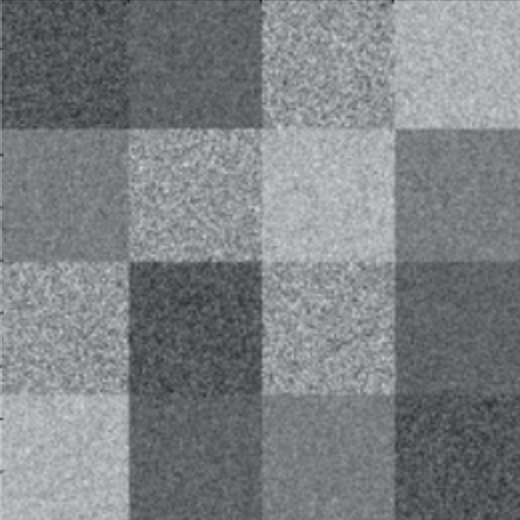
\includegraphics[height = \linewidth]{squares}\par
	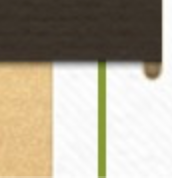
\includegraphics[height = \linewidth]{test}\
	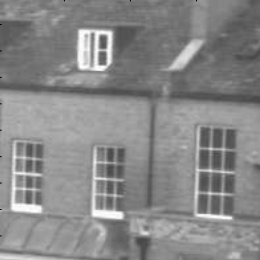
\includegraphics[height = \linewidth]{house}\
	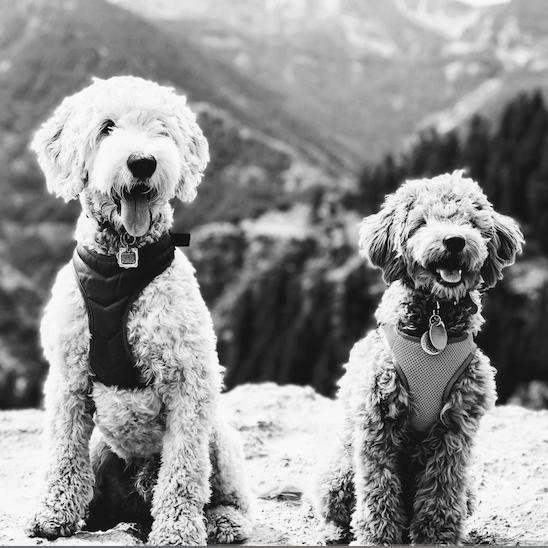
\includegraphics[height = \linewidth]{targetpractice}\par
\end{multicols}
\caption{The images used for training}
\end{center}
\end{figure}

\section{Methods}
Below is a simple overview of the algorithm proposed and then the modified algorithm we implemented.
A more in depth explanations of each step along with descriptions of the associated implementation and difficulties follow the algorithm.

\begin{enumerate}
	\item Randomly initialize the parameters for the MRF and number of classes
	\item Get the most likely segmentation given the MRF parameters
	\item Sample updated noise parameters $\mu$ and $\sigma$ for each class using Metropolis Hastings
	\item Sample updated MRF parameters $\beta_0$ and $\beta_1$ for each class using Metropolis Hastings
	\item Sample number of classes
	\item Repeat steps (2) - (5)
\end{enumerate}
The sampling method follows the same basic pattern: sample new parameters from their prior distributions, calculate an acceptance probability (or likelihood) for those parameters, and then use the Metropolis-Hastings algorithm to choose to accept/reject those parameters.

On the surface, this algorithm is simple. However, many of the equation definitions and notational choices were unclear and required extensive interpretation.
Further, some of the equations as defined in the text suffered from under and overflow errors and thus required considerable reworking to be suitable for implementation.
Sampling the number of classes was the most complex section of the paper and the notation was especially difficult to understand.
As such, we were unable to implement this step, but because the number of classes was a fixable parameter, this was not a significant issue.
Leaving this step out, we implemented the following method.
\begin{enumerate}
	\item Set the number of desired classes and randomly initialize the parameters for the MRF
	\item Get the most likely segmentation given the MRF parameters
	\item Sample updated noise parameters $\mu$ and $\sigma$ for each class using Metropolis Hastings
	\item Sample updated MRF parameters $\beta_0$ and $\beta_1$ for each class using Metropolis Hastings
	\item Repeat steps (2) - (4)
\end{enumerate}

<<<<<<< HEAD

Here is an overview of the variables used in the equations:
=======
\subsection{Variable Definitions}
We define the following variables to use in the various equations to follow:
>>>>>>> 9ce353e61d122320755b9d41ce2216e048ce5122

\begin{itemize}
	\item $\Omega$: The image being classified
	\item $s$: A pixel of the image $\Omega$
	\item $Y$: The grayscale image intensities
	\item $y_{s}$: The grayscale intensity at pixel $s$ in the interval $(0,1]$
	\item $X$: The segmentation labels for the MRF
	\item $x_{s}$: The label to which pixel $s$ is assigned
	\item $\Lambda$: The set of class labels
	\item $\eta_{s}$: The set of 4 direct neighbors of pixel $s$
	\item $\Psi$: The parameter vector consisting of both noise and MRF parameters
	\item $\Theta_{c}$: The noise model parameter vector consisting of $\mu_{c}$ and $\sigma_{c}$
	\item $\beta_{c}^{(0)}$: The external field parameter
	\item $\beta_{c}^{(1)}$: The inter-pixel interaction strength parameter
	\item $T_{t}$: The annealing temperature at iteration $t$
	\item $n_{c}$: The number of pixels of class $c$
	\item $n_{(c, \eta)}$: Abusive notation explained in Section 3.3
\end{itemize}



\subsection{Segment the Image with the MRF}
With an initial set of random parameters to define our MRF, we needed to first find the probability of each pixel being in each class:
\begin{equation}
\begin{aligned}
p\left(x_{s} = c | y_{s}, \eta_{s}, \Psi_{c}\right) & \propto \\
&\frac{1}{\sqrt{2 \pi \sigma_{c}^{2} T_{t}}} \exp \left\{ -\frac{1}{T_{t}} \left[\frac{1}{2} \left(\frac{y_{s}-\mu_{c}}{\sigma_{c}}\right)^{2} + \left( \beta_{c}^{(0)} + \beta^{(1)} V(c, \eta_{s}) \right) \right] \right\}
\end{aligned}
\end{equation}
where $V(c, \eta)=\frac{1}{4} \sum_{t \in \eta}(c \oplus\left.x_{t}\right),$ where $\oplus$ is an operator defined to take the value -1 if its arguments are equal and 1 otherwise.

We then calculated the probabilities over the entire image for each class and took the argmax, thereby assigning each pixel to the class to which it most likely belongs.
The implementation of this process was relatively straightforward and required no adjustments to the equations.


\subsection{Update Noise Parameters}
The noise parameters $\mu_{c}$ and $\sigma_{c}$ are sampled using Metropolis-Hastings with the following likelihood:
\begin{equation}
\begin{aligned}
p\left(\mu_{c}, \sigma_{c} | Y, X\right) & \propto \prod_{s: x_{s}=c} p\left(y_{s} | \mu_{c}, \sigma_{c}\right) p_{r}\left(\mu_{c}\right) p_{r}\left(\sigma_{c}\right) \\
&=\frac{1}{\sigma_{c}\left(2 \pi \sigma_{c}^{2} T_{t}\right)^{n_{c}}} \exp \left\{-\frac{1}{2 T_{t}} \sum_{s: a_{s=c}}\left(\frac{y_{s}-\mu_{c}}{\sigma_{c}}\right)^{2}\right\}
\end{aligned}
\end{equation}

With a firm grasp on Metropolis-Hastings, we expected updating the noise parameters to be straightforward. However, the suggested $T_{t}$ from the paper was so large, we ran into immediate underflow errors during computation.
We soon realized the issue was the $n_{c}$ exponent in the denominator causing our underflow.
While segmenting a small 100 x 100 image into 4 classes, $n_{c}$ should be about 25,000 and possibly much larger.
This necessitated that we calculate the equation in a completely different form which we give below.

\begin{equation}
\begin{aligned}
p\left(\mu_{c}, \sigma_{c} | Y, X\right) & \propto \frac{1}{\sigma_{c}}\prod_{s: x_{s}=c} \frac{1}{2 \pi \sigma_{c}^{2} T_{t}} \exp \left\{-\frac{1}{2 T_{t}} \left(\frac{y_{s}-\mu_{c}}{\sigma_{c}}\right)^{2} \right\}
\end{aligned}
\end{equation}

This allowed us to avoid the exponent and the large sum, both of which could cause massive underflow by calculating a each part of the product individually.
Because this probability would be used only for the acceptance ratio $a$ in the Metropolis-Hastings algorithm, we extended this calculation one step further.

\begin{equation}
\begin{aligned}
a & = \frac{p\left(\mu_{c}^{new}, \sigma_{c}^{new} | Y, X\right)}{p\left(\mu_{c}, \sigma_{c} | Y, X\right)}\\ & \propto \prod_{s: x_{s}=c}  \frac{\frac{1}{2 \pi \sigma_{c}^{new2} T_{t}} \exp \left\{-\frac{1}{2 T_{t}} \left(\frac{y_{s}-\mu_{c}^{new}}{\sigma_{c}^{new}}\right)^{2} \right\}}{\frac{1}{2 \pi \sigma_{c}^{2} T_{t-1}} \exp \left\{-\frac{1}{2 T_{t-1}} \left(\frac{y_{s}-\mu_{c}}{\sigma_{c}}\right)^{2} \right\}}\\
&= \prod_{s: x_s = c} \left( \frac{\sigma_c}{\sigma_c^{new}} \right)^{3} \left( \frac{T_{t-1}}{T_t} \right) \exp \left\{ \frac{-1}{2 T_t} \left( \frac{y_s - \mu_c^{new}}{\sigma_c^{new}} \right)^2 + \frac{1}{2 T_{t-1}} \left( \frac{y_s - \mu_c}{\sigma_c} \right)^2  \right\}
\end{aligned}
\end{equation}

This allowed us to calculate the acceptance ratio for a single pixel before taking the product over all of the pixels of the specified class.
By doing so, we completely avoided underflow. However, we were only getting acceptance ratios of $0$ and $\infty$.
At first this concerned us but we realized that given model parameters, the individual ratios would be very similar (at least across each class) and thus for $a_{s} > 1$ taking the product would approach $\infty$ and for $a_{s} < 1$, the product would approach 0.
Having resolved this issue, we were able to update our noise parameters $\mu_{c}$ and $\sigma_{c}$ properly.

\subsection{Update MRF Parameters}
As in the previous step, the MRF parameters $\beta_{c}^{(0)}$ are sampled using Metropolis-Hastings with the following probability:

\begin{equation}
\begin{array}{l}
p\left(\beta_{c}^{(0)}, c \in \Lambda | X\right) \\
\quad=p\left(X | \beta_{c}^{(0)}, c \in \Lambda\right) p_{r}\left(\beta_{c}^{(0)}, c \in \Lambda\right) \\
\quad=\prod_{\left(c \in \Lambda, _{\eta}\right)}\left(\frac{\exp \left(-\frac{1}{T_{t}}\left[\beta_{c}^{(0)}+\beta^{(1)} V(c, \eta)\right]\right)}{\sum_{i \in \Lambda} \exp \left(-\frac{1}{T_{t}}\left[\beta_{i}^{(0)}+\beta^{(1)} V(i, \eta)\right]\right)}\right)^{n_{(c, \eta)}} \\
\quad=\prod_{(c \in \Lambda)}\left(\frac{\exp \left(-\frac{1}{T_{t}}\left[\beta_{c}^{(0)}\right]\right)}{\sum_{i \in \Lambda} \exp \left(-\frac{1}{T_{t}}\left[\beta_{i}^{(0)}\right]\right)}\right)^{n_{c}} \\
\quad \times \prod_{(c \in \Lambda, \Psi \eta)}\left(\frac{\exp \left(-\frac{1}{T_{t}}\left[\beta^{(1)} V(c, \eta)\right]\right) \sum_{i \in \Lambda} \exp \left(-\frac{1}{T_{t}}\left[\beta_{i}^{(0)}\right]\right)}{\sum_{i \in \Lambda} \exp \left(-\frac{1}{T_{t}}\left[\beta_{i}^{(0)}+\beta^{(1)} V(i, \eta)\right]\right.}\right)^{n_{(c, \eta)}}
\end{array}
\end{equation}

We immediately ran into the issue of the definition of the exponent $n_{(c, \eta)}$ that is used.
The paper defines this as $n_{(c, \eta)}=\#\left(s: x_{s}=c, \eta_{s}=\eta\right)$;
this notation is abusive and does not follow the paper's previously established notational conventions.
As written, this $n$ function takes in a class $c$ and a set of pixels $\eta$, then returns the number of pixels that have label $c$ and neighbors $\eta$.
However, due to the way $\eta$ is defined at the beginning of the paper, each pixel will have a unique set of neighbors.

Thus, this $n$ function will return a 1 if there is a pixel in class $c$ with the given set of neighbors $\eta$ and a $0$ if there is not a pixel in class $c$ with that exact set of neighbors.
Then for each class, iterating over all $\eta_s$ with the $n$ function is equivalent to iterating over all $s: x_s = c$ with the indicator function $\mathbbm{1}(s,c)_{x_s = c}$.
This leads to probabilities corresponding to pixels such that $x_{s} \neq c$ being set to $1$ and essentially excluded from the product, so we remedied this equation as follows:

\begin{equation}
\begin{aligned}
p\left(\beta_{c}^{(0)}, c \in \Lambda | X\right) & = \prod_{s:x_{s} = c}\frac{\exp \left(-\frac{1}{T_{t}}\left[\beta_{c}^{(0)}+\beta^{(1)} V(c, \eta_{s})\right]\right)}{\sum_{i \in \Lambda} \exp \left(-\frac{1}{T_{t}}\left[\beta_{i}^{(0)}+\beta^{(1)} V(i, \eta_{s})\right]\right)}
\end{aligned}
\end{equation}

This greatly simplified the calculations for updating the MRF parameters  $\beta_{c}^{(0)}$.
We used the same method as described in Section 3.2 of calculating each of the individual acceptance ratios $a_{s}$ before taking the product over all the ratios.
A similar equation is proposed for the likelihood $p(\beta_{c}^{(1)}, c \in \Lambda | X)$. However, the paper states that the posterior density calculation for $\beta_{c}^{(1)}$ will not be proper under particular underlying label map configurations.
The paper fixes a value \textit{a priori} of $1.5$ for $\beta_{c}^{(1)}$.
We follow this practice in our approach.

\subsection{Number of classes}
The most difficult part of this paper involved sampling the number of classes.
The notation throughout this sections was very difficult to understand.
Below is the equation for the acceptance ratio for splitting a class $c$ into $c_{1}$ and $c_{2}$.

\begin{equation}\label{acc_prob_num_classes}
\begin{aligned}
\frac{p\left(X=x^{+}, \Psi^{+}, k^{+} | Y=y\right)}{p(X=x, \Psi, k | Y=y)} & \frac{1}{p_{\beta}\left(u_{1}\right) p_{\beta}\left(u_{2}\right) p_{\beta}\left(u_{3}\right)} \\
\times \frac{\partial\left(\Psi_{c 1}, \Psi_{c 2}\right)}{p(\text {segmentation})} &\left|\frac{1}{\partial\left(\Psi_{c}, u_{1}, u_{2}, u_{3}\right)}\right|
\end{aligned}
\end{equation}

<<<<<<< HEAD
Unfortunately, we were never able to work out the notation in a way that made enough sense to even try to implement this sampling.
However, this step only helps find the optimal number of classes for the segmentation, and omitting this step should not affect any other sampling or the performance of the algorithm as a whole.
=======
Unfortunately, we were not able to calculate this acceptance ratio.
The problem arose from the approximation of the first term, which is calculated via
\begin{equation}
\begin{aligned}
   p(X=x, \Psi, k | Y = y) \propto \prod_{s \in \Omega}  \frac{1}{\sqrt{2 \pi \sigma_{x_s}^2}} \exp \left \{ -\frac{1}{2} \left( \frac{y_s - \mu_{x_s} }{ \sigma_{x_s}}\right)^2  \right \} \\
   \times \prod_{s \in \Omega} \frac{\exp \left \{ - \left(\beta_{x_s}^{(0)} + \beta^{(1)} V(x_s, \eta_s) \right)  \right \} }{\sum_{c \in \Lambda} \exp \left \{ -(\beta^{(0)}_c + \beta^{(1)} V(c, \eta_s)  \right \}} \\
   \times p_r\left(\beta^{(1)}\right) p_r(k) \prod_{c \in \Lambda} p_r (\mu_c) p_r ( \sigma_c ) p_r (\beta_c^{(0)}).
\end{aligned}
\end{equation}

When calculating this term, the products over all $ s \in \Omega $ create problems.
In a relatively small 100 x 100 pixel image, this is a product over 10,000 terms.
So, this almost always leads to numerical overflow (i.e. $p(X=x, \Psi, k | Y = y) = \pm \infty $) or underflow (i.e. $ p(X=x, \Psi, k | Y = y) = 0$).
Overflow can be dealt with in certain situations; sometimes we can just leave it be, especially when computing acceptance probabilities, where anything greater than 1 is just taken to be 1.
However, in this case, substituting either $\pm\infty$ or $ 0 $ into (\ref{acc_prob_num_classes}) gives $ \frac{\infty}{\infty} $ or $ \frac{0}{0} $ in the first term, both of which are undefined.

Because of this, we chose not to sample the number of classes in our algorithm.
Fortunately, this step only helps find the optimal number of classes for the segmentation at each step and ommitting this step should not affect the other steps or performance of the algorithm as a whole.
>>>>>>> 7cfea4dc04fc311ee93d7b722a6830ba13fad28a
With this step omitted from the algorithm, we simply specify the desired number of classes before running it.

\section{Results}

We were really shocked that we were able to successfully implement this images segmentation from the paper.
We were not able to achieve the same results as the authors of the paper.
This could be due to our lack of understanding as to what how the different parameters interact and affect the model.
This could be a major factor in determining the variances for the distributions from which the proposed $\mu_{c}$ and $\sigma_{c}$ are drawn.

We intially tested our model with the noisy squares image from Figure 1.
The authors used this image in their paper and achieved great results in segmenting the image.
Our model, however, struggled to identify the classes in the same way that the author's method did.
This could be due to not having implemented the part step that resamples the number of classes, but we speculate that this has more to do with unknown parameters that we have set that may not be ideal.
With this image, we noticed that the segmentations would converge to segmentations with only 2 or 3 classes, even when we had specified 5 or more classes, where certain squares were properly segmented but other squares the model seemed to be uncertain.
This resulted in some squares being solid, where other similar squares were different combinations of the 2 or 3 classes the model was identifying.
Below are the results that we were able to achieve compared to the authros' results in the paper.
We were unable to get our model to produce the final smooth result that the paper achieved as shown in Figure 2.
This was the desired output of our model, but unfortunately we were unable to achieve this result.

\begin{figure}[!htb]
\begin{center}
\begin{multicols}{3}
	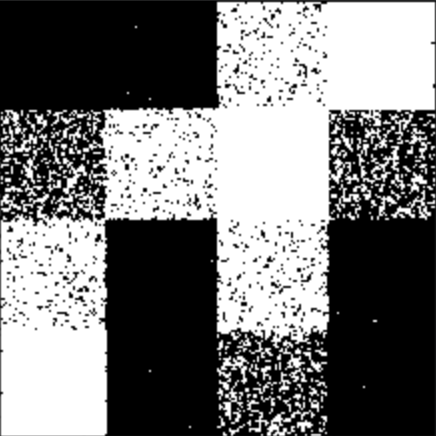
\includegraphics[height = \linewidth]{squares0}\par
    Our result
	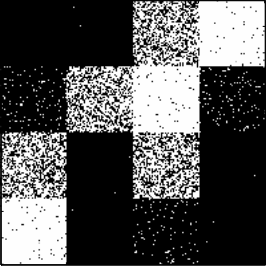
\includegraphics[height = \linewidth]{squares1}\par
    Author's intermediary result
	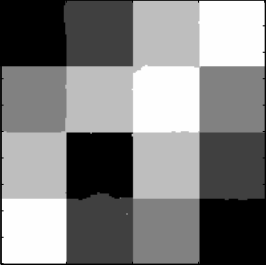
\includegraphics[height = \linewidth]{squares2}\par
    Author's final result
\end{multicols}
\caption{Results comparison for squares image}
\end{center}
\end{figure}

The similarity of our result and their intermediary result is striking and suggests that our model is very close to working, however, our model never showed signs of smoothing out, even with thousands of iterations.

As for the other images we used, this is what the results looked like.
Again our model was able to identify major classes of pixels and segment them, however, our model mostly failed when it came to smoothing classes and removing noise.
This can be seen in both of the examples below.

\begin{figure}[!htb]
\begin{center}
\begin{multicols}{5}
    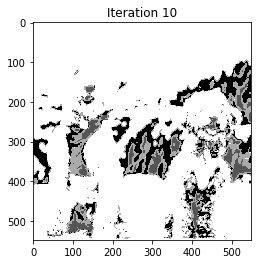
\includegraphics[height = \linewidth]{dogs_10}\par
	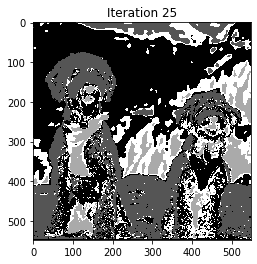
\includegraphics[height = \linewidth]{dogs_25}\par
	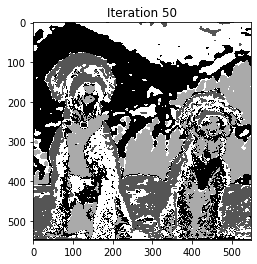
\includegraphics[height = \linewidth]{dogs_50}\par
	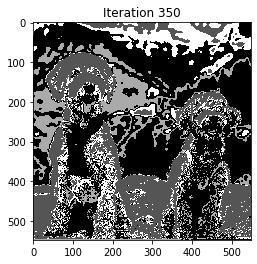
\includegraphics[height = \linewidth]{dogs_350}\par
	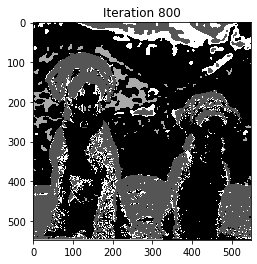
\includegraphics[height = \linewidth]{dogs_800}\par
\end{multicols}

\begin{multicols}{5}
    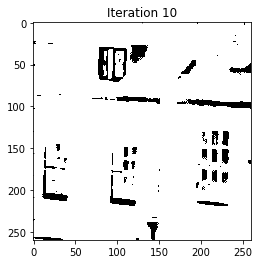
\includegraphics[height = \linewidth]{house_10}\par
	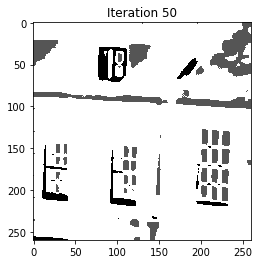
\includegraphics[height = \linewidth]{house_50}\
	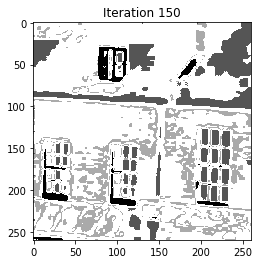
\includegraphics[height = \linewidth]{house_150}\par
	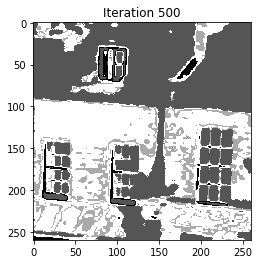
\includegraphics[height = \linewidth]{house_500}\
	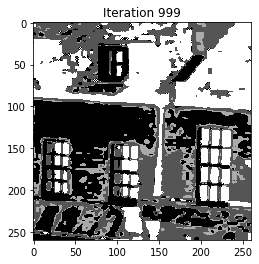
\includegraphics[height = \linewidth]{house_1000}\par
\end{multicols}

\caption{The images used for training}
\end{center}
\end{figure}


\section{Comparison to Other Methods}
As part of our analysis, we wanted to compare our model to classical machine learning image segmentation approaches.
For this we used K-means and pixel threshold testing.
Throughout our model, we typically used 4 classes from which our model sampled, thus for our K-means we used 4 classes.
Here is the K-means segmented output compared to our MRF output.

\begin{figure}[!htb]
\begin{center}
\begin{multicols}{4}
	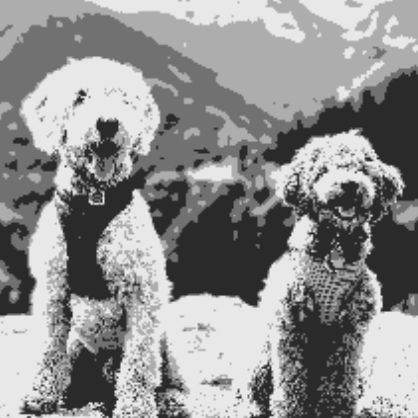
\includegraphics[width = \linewidth]{kmeans}\par
    K-means with 4 clusters
	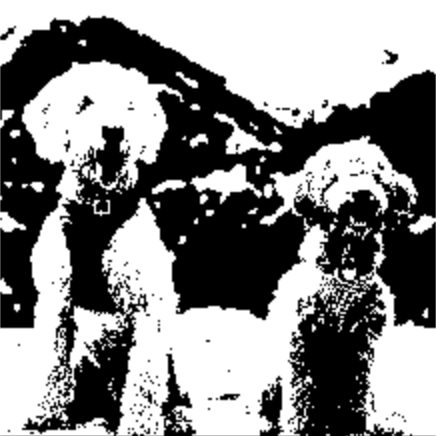
\includegraphics[width = \linewidth]{thresh1}\par
    2-class pixel thresholding
	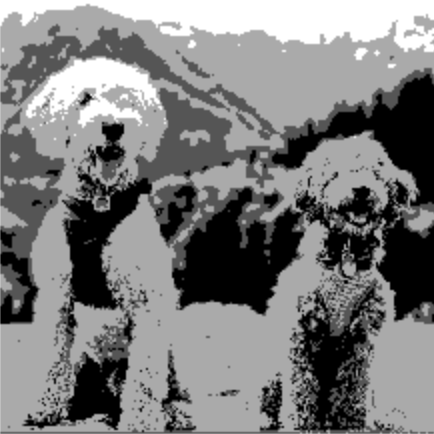
\includegraphics[width = \linewidth]{threshold}\par
    4-class pixel thresholding
	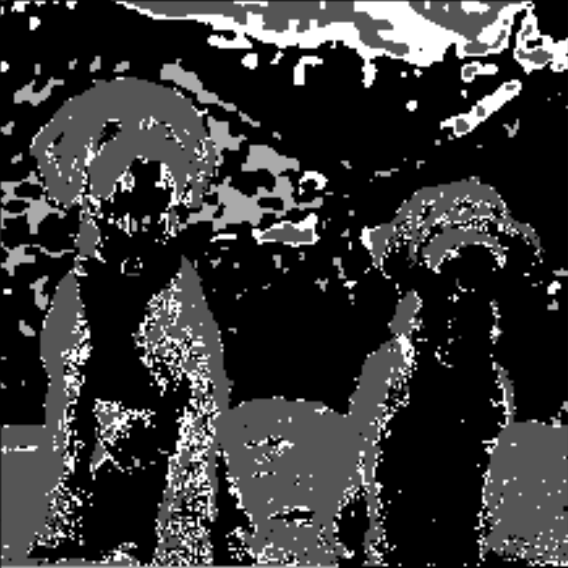
\includegraphics[width = \linewidth]{clustered}\par
    Model results after 800 iterations
\end{multicols}
\caption{Comparison to other methods}
\end{center}
\end{figure}


We also wanted to do some other comparisons, so we utilized the scikit learn image segmentation library to divide segment the imagebased on thresholds.
To do this, we first chose to do a 2-class threshold using the mean pixel brightness.
All of the pixels brighter than the mean were assigned to one cluster and the rest to the other.
We then tried thresholding with 4 classes by assigning labels based on quartiles of pixel brightness.
The bottom 25\% of pixels belonged to the first class and so on.


\section{Analysis}
Our methods turned out to be fairly effective.
It was able to identify different classes initially and improve them, although it was only a slight improvement.
Our model cannot compete with current state of the art methods.
However, had our model been able to smooth out classes as we expected it to (see Figure 2), its performance likely would have been on par with newer state of the art methods.

The results we achieved with the squares image reflected exactly the results that the authors had achieved in the paper.
Our model seemed to work exactly as theirs had.
However, we were unable to tune our model so that it would smooth out each cluster and achieve a result similar to the Author's final result.
This was the main issue with our model in all cases.

We saw the same results with the image of the side of a building that was also used in the paper (see Figure 3), but again, our results never smoothed out like theirs did.
This is not to say that our model failed completely to smooth out classes.
When comparing our model side by side with K-means and thresholding techniques, we noticed that our results were much closer to the results from these methods.
It is hard to say whether our model was able to smooth these boundaries better than the other methods, especially because although the classes are very similar among methods, they are represented with different colors making it hard to compare them.
In the 4-class pixel thresholding image, we notice that the labels for the dog on the left are split over his face (see Figure 4) even though the pixels were very close in intensity.
Our model, like the K-means, was able to adjust the classes to account for more similar pixels instead of a more uniform partitioning.

Perhaps the most notable is the black labeling of the dog on the right from our model.
Our model has grouped together a few clusters and grouped them together, something that none of the other models were able to do.
Even then, our model seems to be mostly classified into 2 classes, and is most similar to the 2-class pixel thresholding result, which is similar to the results we were seeing when classifying the squares image.


\section{Conclusion}
Although our model did work, it seemed to represent striking similarities to other rudimentary techniques like K-means and pixel thresholding.
While this is not an issue, we expected that after more iterations, the classes would smooth out and we would see less noise and better groups of classes in our segmentations.
The authors of the paper we used achieved near exact results to those that we found, however, with enough training, their results seemed to improve to what we would have expected, while our model did not.
This was most likely due to poor choices for our parameters, especially those defining the prior dristributions from which other parameters were drawn.
Without a stronger understanding of what these parameters were doing, it was hard to know why we were getting poor results.
This could also be a result of not having implemented the full method as was done in the paper, although this seems less likely to us than having poor parameters.

Implementing the method for sampling the number of classes in each iteration does not seem feasible given only the information provided in the paper.
Thus, for future work to improve this model, a major grid search over many different images could be implemented to try and identify the best parameters for the model.
This would require a vast amount of computing power, as there are at least 5 different parameters that are arbitrarily chosen.

Overall, we are very happy with the work we were able to do on this project, even though the results are not amazing.
Just getting the model to work properly was a great achievement for us as there was a lot of work required to both understand and then implement the equations and methods explained in the paper.

\end{document}
